\documentclass[aspectratio=169]{beamer}
\usetheme{default}
\usepackage[utf8]{inputenc}
\usepackage[T1]{fontenc}
\usepackage{lmodern}
\usepackage{tikz}
\usetikzlibrary{positioning,arrows.meta}
\usepackage{tabularx,booktabs}
\usepackage{hyperref}
\usepackage{listings}
\usepackage{xcolor}
\usepackage{ragged2e}

\definecolor{courseblue}{RGB}{28,92,142}
\definecolor{courseblue2}{RGB}{21,73,116}
\definecolor{courselight}{RGB}{238,244,250}
\definecolor{coursegray}{RGB}{105,115,125}

\setbeamertemplate{navigation symbols}{}
\setbeamertemplate{headline}{}
\setbeamertemplate{frametitle}{%
  \nointerlineskip%
  \begin{beamercolorbox}[wd=\paperwidth,ht=0.55cm,dp=0.12cm,leftskip=0.2cm]{frametitle}
    \usebeamerfont{frametitle}\insertframetitle
  \end{beamercolorbox}}
\setbeamercolor{frametitle}{fg=white,bg=courseblue}
\setbeamercolor{title}{fg=white}
\setbeamerfont{title}{series=\bfseries,size=\Large}
\setbeamercolor{normal text}{fg=black,bg=white}
\setbeamerfont{footline}{size=\tiny}
\setbeamercolor{footline}{fg=white,bg=courseblue2}
\setbeamertemplate{footline}{%
  \hbox{%
    \begin{beamercolorbox}[wd=.22\paperwidth,ht=0.22cm,dp=0.05cm,leftskip=0.15cm]{footline}Setup Tutorial\end{beamercolorbox}%
    \begin{beamercolorbox}[wd=.62\paperwidth,ht=0.22cm,dp=0.05cm,center]{footline}Class 2 --- Setting Up Python\end{beamercolorbox}%
    \begin{beamercolorbox}[wd=.16\paperwidth,ht=0.22cm,dp=0.05cm,rightskip=0.15cm plus 1fil]{footline}\insertframenumber/\inserttotalframenumber\end{beamercolorbox}%
  }}

\setbeamertemplate{itemize item}{\textcolor{courseblue}{$\blacktriangleright$}}
\setbeamertemplate{itemize subitem}{\textcolor{courseblue}{$\triangleright$}}
\setbeamertemplate{enumerate item}{\textcolor{courseblue}{\insertenumlabel.}}

\lstdefinestyle{coursebash}{
  basicstyle=\ttfamily\scriptsize,
  breaklines=true,
  frame=single,
  backgroundcolor=\color{gray!6},
  rulecolor=\color{gray!35},
  xleftmargin=0.05cm,
  xrightmargin=0.05cm,
  columns=fullflexible,
  keepspaces=true
}
\lstdefinestyle{coursepython}{
  language=Python,
  basicstyle=\ttfamily\scriptsize,
  breaklines=true,
  frame=single,
  backgroundcolor=\color{gray!6},
  rulecolor=\color{gray!35},
  xleftmargin=0.05cm,
  xrightmargin=0.05cm,
  columns=fullflexible,
  keepspaces=true
}

\tikzset{
  flowbox/.style={draw=courseblue, rounded corners=2pt, thick, fill=white, align=center, minimum height=0.7cm, minimum width=1.8cm, font=\scriptsize},
  accentbox/.style={draw=courseblue2, rounded corners=2pt, thick, fill=courselight, align=center, minimum height=0.7cm, minimum width=1.8cm, font=\scriptsize\bfseries},
  arrow/.style={-Latex, thick, draw=courseblue}
}

\newcommand{\coursefooter}{}
\newcommand{\coursename}{}
\newcommand{\learninggoals}[1]{\begin{block}{By the end of this class, you should be able to}#1\end{block}}
\newcommand{\repoactivity}[1]{\begin{block}{Repository activity}#1\end{block}}
\newcommand{\readinglist}[1]{\begin{block}{Useful references}\footnotesize #1\end{block}}
\newcommand{\coursecontextframe}[4]{
\begin{frame}{Course context}
\begin{block}{#1}#2\end{block}
\begin{itemize}
\item #3
\item #4
\end{itemize}
\coursefooter
\end{frame}}
\newcommand{\classclosingframe}[4]{
\begin{frame}{Take-home messages}
#1
\begin{block}{Before next class}#2\end{block}
\begin{itemize}
\item #3
\item #4
\end{itemize}
\coursefooter
\end{frame}}


\title{Class 2: Setting Up Python}
\author{}
\date{}

\begin{document}

\begin{frame}[plain]
\vspace{1.2cm}
\begin{center}
\begin{beamercolorbox}[wd=0.92\paperwidth,ht=0.9cm,dp=0.25cm,center,rounded=true]{frametitle}
{\Large\bfseries Class 2: Setting Up Python}
\end{beamercolorbox}
\vspace{1.1cm}
{\large Python environment, Jupyter, VS Code, and virtual environments}
\end{center}
\end{frame}

\begin{frame}{Agenda}
\begin{itemize}
\item Install Python and check that it works from the terminal.
\item Install Visual Studio Code and the Python/Jupyter extensions.
\item Create an isolated project environment with \texttt{venv}.
\item Install Jupyter and common Python libraries.
\item Understand the alternative: Miniconda and Conda environments.
\item Run the first script and the first notebook.
\end{itemize}
\coursefooter
\end{frame}

\begin{frame}{Learning goals}
\learninggoals{
\begin{itemize}
\item Explain why local Python projects should use isolated environments.
\item Install and verify Python, pip, VS Code, and Jupyter.
\item Create, activate, use, and deactivate a \texttt{venv} environment.
\item Choose between \texttt{venv} and Miniconda for a basic Python workflow.
\end{itemize}}
\coursefooter
\end{frame}

\coursecontextframe
{From notebooks to real projects}
{In this course, Python is not only used to write small examples: it becomes the environment where data, models, APIs, and dashboards live.}
{A working setup is therefore part of the programming workflow, not an administrative detail.}
{If the environment is reproducible, code can be tested, shared, deployed, and debugged much more easily.}

\begin{frame}{The full setup}
\begin{block}{Main idea}
We create one clean project folder with its own Python interpreter, its own packages, and its own notebook kernel.
\end{block}
\vspace{0.4em}
\begin{itemize}
\item \textbf{Python} runs the code.
\item \textbf{VS Code} is the editor where we write scripts and notebooks.
\item \textbf{\texttt{my\_first\_env}} is the isolated environment for this project.
\item \textbf{Packages} such as NumPy and pandas are installed inside that environment.
\item \textbf{Jupyter} lets us combine code, text, plots, and results interactively.
\end{itemize}
\coursefooter
\end{frame}

\begin{frame}[fragile]{Step 1 --- Install Python}
\begin{enumerate}
\item Go to the official Python website and download a recent Python 3 version.
\item On Windows, check \textbf{Add python.exe to PATH} before clicking \textbf{Install Now}.
\item On macOS/Linux, Python may already exist, but installing a recent Python 3 version is still recommended.
\item Open a terminal and verify the installation.
\end{enumerate}
\begin{lstlisting}[style=coursebash]
python --version
# or, on some systems:
python3 --version
\end{lstlisting}
\coursefooter
\end{frame}

\begin{frame}[fragile]{Step 2 --- Check pip}
\begin{itemize}
\item \texttt{pip} is the standard tool used to install Python packages.
\item Always check \texttt{pip} from the same Python installation you plan to use.
\end{itemize}
\begin{lstlisting}[style=coursebash]
python -m pip --version
\end{lstlisting}
\begin{block}{Why use \texttt{python -m pip}?}
It reduces confusion when multiple Python versions are installed: the selected Python runs its own package installer.
\end{block}
\coursefooter
\end{frame}

\begin{frame}{Step 3 --- Install Visual Studio Code}
\begin{enumerate}
\item Download and install Visual Studio Code.
\item Open VS Code.
\item Go to the Extensions panel.
\item Install the Microsoft \textbf{Python} extension.
\item Install the Microsoft \textbf{Jupyter} extension.
\end{enumerate}
\begin{block}{Course relevance}
VS Code lets us edit scripts, open terminals, run notebooks, and select the correct Python environment from one place.
\end{block}
\coursefooter
\end{frame}

\begin{frame}[fragile]{Step 4 --- Create a project folder}
\begin{itemize}
\item Keep each project in its own folder.
\item Open a terminal and move into that folder before creating the environment.
\end{itemize}
\begin{lstlisting}[style=coursebash]
mkdir ml_course
cd ml_course
\end{lstlisting}
\begin{block}{Mental model}
Everything we install next belongs to this project, not to the whole computer.
\end{block}
\coursefooter
\end{frame}

\begin{frame}[fragile]{Step 5 --- Create a virtual environment with venv}
\begin{itemize}
\item \texttt{venv} is included with Python.
\item We will call our environment \texttt{my\_first\_env}, so its purpose is visible in the project folder.
\end{itemize}
\begin{lstlisting}[style=coursebash]
python -m venv my_first_env
# or, on some macOS/Linux systems:
python3 -m venv my_first_env
\end{lstlisting}
\begin{block}{Result}
Your project now contains an isolated Python environment inside \texttt{my\_first\_env}.
\end{block}
\coursefooter
\end{frame}

\begin{frame}[fragile]{Step 6 --- Activate the environment}
\begin{columns}[T]
\column{0.48\textwidth}
\textbf{Windows}
\begin{lstlisting}[style=coursebash]
my_first_env\Scripts\activate
\end{lstlisting}
\vspace{0.4em}
\textbf{PowerShell alternative}
\begin{lstlisting}[style=coursebash]
my_first_env\Scripts\Activate.ps1
\end{lstlisting}
\column{0.48\textwidth}
\textbf{macOS/Linux}
\begin{lstlisting}[style=coursebash]
source my_first_env/bin/activate
\end{lstlisting}
\vspace{0.4em}
\textbf{You should see}
\begin{lstlisting}[style=coursebash]
(my_first_env) ...
\end{lstlisting}
\end{columns}
\coursefooter
\end{frame}

\begin{frame}[fragile]{Step 7 --- Install packages}
\begin{itemize}
\item With the environment active, install the libraries needed for the course.
\item These packages are installed inside \texttt{my\_first\_env}, not globally.
\end{itemize}
\begin{lstlisting}[style=coursebash]
python -m pip install numpy pandas matplotlib scikit-learn
\end{lstlisting}
\begin{lstlisting}[style=coursebash]
python -m pip list
\end{lstlisting}
\begin{block}{Why not just \texttt{pip install ...}?}
\texttt{pip install ...} may use a different Python if several versions or environments exist. \texttt{python -m pip ...} says explicitly: install into the Python environment I am currently running.
\end{block}
\coursefooter
\end{frame}

\begin{frame}[fragile]{Step 8 --- Install Jupyter}
\begin{itemize}
\item Jupyter lets us write code, text, formulas, and plots in the same document.
\item JupyterLab is the modern notebook interface.
\end{itemize}
\begin{lstlisting}[style=coursebash]
python -m pip install jupyterlab
jupyter lab
\end{lstlisting}
\begin{block}{First check}
Create a notebook, select the project kernel, and run \texttt{print("Hello world!")}.
\end{block}
\coursefooter
\end{frame}

\begin{frame}[fragile]{Step 9 --- Test Python in a notebook}
\begin{lstlisting}[style=coursepython]
import numpy as np

x = np.array([1, 2, 3, 4])
print(x)
print(x.mean())
\end{lstlisting}
\begin{block}{Expected output}
If the cell runs and prints \texttt{2.5}, Python, NumPy, Jupyter, and the environment are working together.
\end{block}
\coursefooter
\end{frame}

\begin{frame}{Step 10 --- Select the environment in VS Code}
\begin{enumerate}
\item Open the project folder in VS Code.
\item Open the command palette: \texttt{Ctrl/Cmd + Shift + P}.
\item Search for \texttt{Python: Select Interpreter}.
\item Choose the interpreter inside \texttt{my\_first\_env}.
\item For notebooks, click \textbf{Select Kernel} and choose the same environment.
\end{enumerate}
\begin{block}{Important}
The terminal, Python scripts, and notebooks should all use the same environment.
\end{block}
\coursefooter
\end{frame}

\begin{frame}[fragile]{Step 11 --- Run the first Python script}
\begin{itemize}
\item Create a file called \texttt{hello.py}.
\item Write a few lines of Python.
\item Run it from the VS Code terminal.
\end{itemize}
\begin{lstlisting}[style=coursepython]
name = "Alice"
print("Hello", name)
\end{lstlisting}
\begin{lstlisting}[style=coursebash]
python hello.py
\end{lstlisting}
\coursefooter
\end{frame}

\begin{frame}[fragile]{Step 12 --- Deactivate and reactivate}
\begin{itemize}
\item When finished, deactivate the environment.
\item The environment is not deleted: it is only switched off.
\end{itemize}
\begin{lstlisting}[style=coursebash]
deactivate
\end{lstlisting}
\begin{block}{Next time}
Return to the project folder and activate \texttt{my\_first\_env} again before working.
\end{block}
\coursefooter
\end{frame}

\begin{frame}{Alternative: Miniconda}
\begin{itemize}
\item Miniconda is a small Python distribution with the \texttt{conda} environment manager.
\item It is very common in data science and scientific computing.
\item It can manage Python versions and complex binary dependencies.
\item It is slightly heavier conceptually than \texttt{venv}, but useful for scientific Python stacks.
\end{itemize}
\begin{block}{Practical rule}
Use \texttt{venv} for simple Python projects; consider Conda when scientific dependencies become difficult to install.
\end{block}
\coursefooter
\end{frame}

\begin{frame}[fragile]{Creating a Conda environment}
\begin{lstlisting}[style=coursebash]
conda create -n mlcourse python=3.13
conda activate mlcourse
conda install numpy pandas matplotlib scikit-learn jupyter
jupyter lab
\end{lstlisting}
\begin{block}{Same idea, different tool}
Both \texttt{venv} and Conda create isolated environments. The goal is the same: make the project reproducible and avoid dependency conflicts.
\end{block}
\coursefooter
\end{frame}

\begin{frame}{venv versus Miniconda}
\begin{columns}[T]
\column{0.48\textwidth}
\textbf{venv}
\begin{itemize}
\item Included with Python.
\item Uses \texttt{pip}.
\item Lightweight and simple.
\item Good first option for teaching.
\end{itemize}
\column{0.48\textwidth}
\textbf{Miniconda}
\begin{itemize}
\item Separate installation.
\item Uses \texttt{conda} and sometimes \texttt{pip}.
\item More features for scientific stacks.
\item Useful for complex scientific dependencies.
\end{itemize}
\end{columns}
\coursefooter
\end{frame}

\begin{frame}{Common problems and quick fixes}
\begin{itemize}
\item \textbf{\texttt{python} not found}: check PATH, try \texttt{python3}, or reinstall Python.
\item \textbf{Package not found}: activate the environment and install the package there.
\item \textbf{Notebook uses wrong packages}: select the correct Jupyter kernel.
\item \textbf{Activation blocked on Windows}: use Command Prompt or adjust PowerShell execution policy for local scripts.
\end{itemize}
\coursefooter
\end{frame}

\begin{frame}{Everyday workflow}
\centering
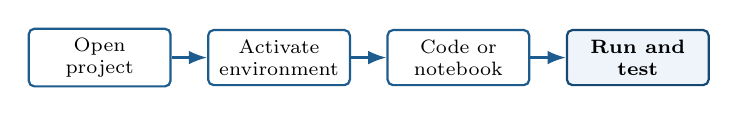
\begin{tikzpicture}[node distance=0.45cm and 0.45cm]
\node[flowbox] (folder) {Open\\project};
\node[flowbox, right=of folder] (activate) {Activate\\environment};
\node[flowbox, right=of activate] (code) {Code or\\notebook};
\node[accentbox, right=of code] (run) {Run and\\test};
\foreach \a/\b in {folder/activate,activate/code,code/run}{\draw[arrow] (\a) -- (\b);}
\end{tikzpicture}
\vspace{1em}
\begin{block}{The habit to build}
Never install packages randomly. First activate the project environment, then install and run code there.
\end{block}
\coursefooter
\end{frame}

\begin{frame}{Questions you should be able to answer}
\begin{itemize}
\item Why should every Python project have its own environment?
\item What is the difference between Python, pip, VS Code, and Jupyter?
\item How do you create and activate a \texttt{venv} environment?
\item How do you install a package in the active environment?
\item When might Miniconda be useful instead of \texttt{venv}?
\end{itemize}
\coursefooter
\end{frame}

\begin{frame}{Discussion prompt}
\begin{block}{Question}
A model works on your laptop, but not on a colleague's machine. What could have gone wrong?
\end{block}
\begin{itemize}
\item Different Python versions.
\item Missing or incompatible packages.
\item Wrong VS Code interpreter or notebook kernel.
\item No documented environment setup.
\end{itemize}
\coursefooter
\end{frame}

\begin{frame}{Papers and materials}
\readinglist{
\href{https://www.python.org/downloads/}{Python downloads};\
\href{https://code.visualstudio.com/}{Visual Studio Code};\
\href{https://docs.python.org/3/library/venv.html}{Python venv documentation};\
\href{https://jupyter.org/install}{Jupyter installation guide};\
\href{https://docs.conda.io/}{Conda documentation}.
}
\coursefooter
\end{frame}

\classclosingframe
{\begin{itemize}
\item A reliable Python workflow starts with a reproducible Python environment.
\item \texttt{venv} is the simplest way to isolate packages for one project.
\item VS Code and Jupyter must point to the same environment to avoid confusion.
\item Miniconda is a useful alternative, especially for scientific Python dependencies.
\end{itemize}}
{Install Python, create one project folder, activate an environment, and run one notebook successfully.}
{Once this works, we can move from setup to real data handling.}
{The next step is using pandas to load, inspect, clean, and visualize data.}

\end{document}
